\documentclass[aspectratio=169,12pt,t]{beamer}

% --- Theme: Metropolis (modern, clean) ---
\usetheme[progressbar=frametitle,numbering=fraction,block=fill]{metropolis}

% --- Fira Sans font (install texlive-fonts-extra if missing) ---
\IfFileExists{FiraSans.sty}{\usepackage[sfdefault]{FiraSans}}{}

% --- Light background with warm accent ---
\definecolor{mDarkTeal}{RGB}{35,55,59}
\definecolor{mLightBrown}{RGB}{235,228,216}
\definecolor{mAccent}{RGB}{140,70,20}

\setbeamercolor{normal text}{fg=mDarkTeal,bg=white}
\setbeamercolor{alerted text}{fg=mAccent}
\setbeamercolor{frametitle}{bg=mDarkTeal,fg=white}
\setbeamercolor{progress bar}{fg=mAccent,bg=mLightBrown}
\setbeamercolor{title separator}{fg=mAccent}
\setbeamercolor{progress bar in head/foot}{fg=mAccent,bg=mLightBrown}
\setbeamercolor{progress bar in section page}{fg=mAccent,bg=mLightBrown}

% --- Packages ---
\usepackage[utf8]{inputenc}
\usepackage{amsmath,amssymb,amsthm}
\usepackage{mathrsfs}
\usepackage{tikz}
\usetikzlibrary{arrows.meta,positioning,calc,decorations.pathreplacing,shapes,patterns}
\usepackage{pgfplots}
\pgfplotsset{compat=1.18}

% --- Custom colors for content types ---
\definecolor{defcolor}{RGB}{25,85,120}
\definecolor{thmcolor}{RGB}{140,35,35}
\definecolor{proofcolor}{RGB}{35,100,50}
\definecolor{excolor}{RGB}{140,75,10}
\definecolor{remcolor}{RGB}{90,90,90}

% --- Beamer blocks for mathematical content types ---
% Override Metropolis block styling for colored blocks
\newenvironment{defblock}[1]{%
  \setbeamercolor{block title}{bg=defcolor,fg=white}%
  \setbeamercolor{block body}{bg=defcolor!5}%
  \begin{block}{#1}}{\end{block}}

\newenvironment{thmblock}[1]{%
  \setbeamercolor{block title}{bg=thmcolor,fg=white}%
  \setbeamercolor{block body}{bg=thmcolor!5}%
  \begin{block}{#1}}{\end{block}}

\newenvironment{proofblock}[1]{%
  \setbeamercolor{block title}{bg=proofcolor,fg=white}%
  \setbeamercolor{block body}{bg=proofcolor!5}%
  \begin{block}{#1}}{\end{block}}

\newenvironment{exblock}[1]{%
  \setbeamercolor{block title}{bg=excolor,fg=white}%
  \setbeamercolor{block body}{bg=excolor!5}%
  \begin{block}{#1}}{\end{block}}

\newenvironment{remblock}[1]{%
  \setbeamercolor{block title}{bg=remcolor,fg=white}%
  \setbeamercolor{block body}{bg=remcolor!5}%
  \begin{block}{#1}}{\end{block}}

% --- Metadata ---
\title{Chapter 1: The Real and Complex Number Systems}
\subtitle{Section: Ordered Sets}
\author{Based on Walter Rudin's \emph{Principles of Mathematical Analysis}}
\date{}

\begin{document}

% ============================================================
% TITLE AND OUTLINE
% ============================================================
\begin{frame}
  \titlepage

  \note{
    Welcome back to the Principles of Mathematical Analysis video series.
    This is Chapter 1, Section 2: Ordered Sets. In the previous section, we
    saw that the rational numbers have gaps, and that the set of rationals p
    with p squared less than 2 has no least upper bound in the rationals.
    In this section, we will make these ideas precise by defining what it
    means for a set to be ordered, and what it means for a set to have
    the least-upper-bound property. Let's begin.
  }
\end{frame}

\begin{frame}{Outline}
  \tableofcontents

  \note{
    Here is our plan for this section. We will start with the basic
    definitions of order and ordered sets. Then we will define upper
    bounds, lower bounds, and the supremum and infimum. After exploring
    some key examples, we will introduce the least-upper-bound property
    and prove an important theorem connecting least upper bounds and
    greatest lower bounds.
  }
\end{frame}

% ============================================================
% MOTIVATION
% ============================================================

% --- Build 1/3 ---
\begin{frame}{Why This Section Matters}
  \begin{itemize}
    \item The Introduction showed that $\mathbb{Q}$ has \alert{gaps}
  \end{itemize}

  \note{
    In the previous section, we showed that there is no rational number
    whose square is 2. This revealed a fundamental gap in the rational
    number system. Now we need the language to describe this gap precisely.
  }
\end{frame}

% --- Build 2/3 ---
\begin{frame}{Why This Section Matters}
  \begin{itemize}
    \item The Introduction showed that $\mathbb{Q}$ has \alert{gaps}
    \item We need precise language: \emph{order}, \emph{bounds}, \emph{supremum}
  \end{itemize}

  \note{
    To describe these gaps, we need to formalize the notions of order,
    upper and lower bounds, and the supremum. These are the core concepts
    of this section.
  }
\end{frame}

% --- Build 3/3 ---
\begin{frame}{Why This Section Matters}
  \begin{itemize}
    \item The Introduction showed that $\mathbb{Q}$ has \alert{gaps}
    \item We need precise language: \emph{order}, \emph{bounds}, \emph{supremum}
    \item The \alert{least-upper-bound property} will distinguish $\mathbb{R}$ from $\mathbb{Q}$
  \end{itemize}

  \note{
    The key idea in this section is the least-upper-bound property. This
    is the property that the real numbers have but the rationals do not.
    It will be the foundation for everything that follows in this book.
    Let's start with the basic definitions.
  }
\end{frame}

% ============================================================
\section{Definitions and Setup}
% ============================================================

% --- Definition 1.5: Build 1/3 ---
\begin{frame}{Definition 1.5: Order on a Set}
  \begin{defblock}{Definition 1.5 --- Order}
    Let $S$ be a set. An \alert{order} on $S$ is a relation, denoted by $<$, with:

    \vspace{0.3em}
    \textbf{(i) Trichotomy:} If $x \in S$ and $y \in S$, then exactly one holds:
    \[
      x < y, \qquad x = y, \qquad y < x.
    \]
  \end{defblock}

  \note{
    Let's define what an order is. An order on a set S is a relation,
    written with the less-than symbol, satisfying two properties. The
    first property is called trichotomy: for any two elements x and y
    in S, exactly one of the three statements x less than y, x equals y,
    or y less than x is true. There is no ambiguity --- one and only one
    of these holds.
  }
\end{frame}

% --- Definition 1.5: Build 2/3 ---
\begin{frame}{Definition 1.5: Order on a Set}
  \begin{defblock}{Definition 1.5 --- Order}
    Let $S$ be a set. An \alert{order} on $S$ is a relation, denoted by $<$, with:

    \vspace{0.3em}
    \textbf{(i) Trichotomy:} If $x \in S$ and $y \in S$, then exactly one holds:
    \[
      x < y, \qquad x = y, \qquad y < x.
    \]

    \textbf{(ii) Transitivity:} If $x < y$ and $y < z$, then $x < z$.
  \end{defblock}

  \note{
    The second property is transitivity. If x is less than y and y is
    less than z, then x is less than z. This is the familiar chaining
    property that lets us build up a consistent ordering of elements.
    Together, trichotomy and transitivity are all we need for an order.
  }
\end{frame}

% --- Definition 1.5: Build 3/3 (notation) ---
\begin{frame}{Definition 1.5: Order on a Set}
  \begin{defblock}{Definition 1.5 --- Order}
    Let $S$ be a set. An \alert{order} on $S$ is a relation, denoted by $<$, with:

    \vspace{0.3em}
    \textbf{(i) Trichotomy:} If $x \in S$ and $y \in S$, then exactly one holds:
    \[
      x < y, \qquad x = y, \qquad y < x.
    \]

    \textbf{(ii) Transitivity:} If $x < y$ and $y < z$, then $x < z$.
  \end{defblock}

  \vspace{0.5em}
  \textbf{Notation:} $y > x$ means $x < y$. \quad $x \leq y$ means $x < y$ or $x = y$.

  \note{
    A few words about notation. We write y greater than x as a synonym
    for x less than y. And x less than or equal to y means that either
    x is strictly less than y, or x equals y. In other words, x less
    than or equal to y is the negation of x greater than y. Now let's
    define ordered sets.
  }
\end{frame}

% --- Definition 1.6 ---
\begin{frame}{Definition 1.6: Ordered Set}
  \begin{defblock}{Definition 1.6 --- Ordered Set}
    An \alert{ordered set} is a set $S$ in which an order is defined.
  \end{defblock}

  \vspace{0.5em}
  \textbf{Example:} $\mathbb{Q}$ is an ordered set, where $r < s$ means $s - r$ is a positive rational.

  \note{
    An ordered set is simply a set equipped with an order relation
    satisfying the two properties we just defined. The most familiar
    example is the rational numbers, where r is less than s means that
    s minus r is a positive rational number. You can verify that this
    relation satisfies both trichotomy and transitivity. Now that we
    have ordered sets, let's talk about bounds.
  }
\end{frame}

% --- Definition 1.7 with diagram ---
\begin{frame}{Definition 1.7: Upper and Lower Bounds}
  \begin{defblock}{Definition 1.7 --- Bounded Above}
    Let $S$ be an ordered set and $E \subset S$. If there exists $\beta \in S$ such that
    $x \leq \beta$ for every $x \in E$, then $E$ is \alert{bounded above}, and $\beta$ is an
    \alert{upper bound} of $E$.
  \end{defblock}

  \vspace{0.3em}
  \alert{Lower bounds} are defined symmetrically (with $\geq$ in place of $\leq$).

  \begin{center}
  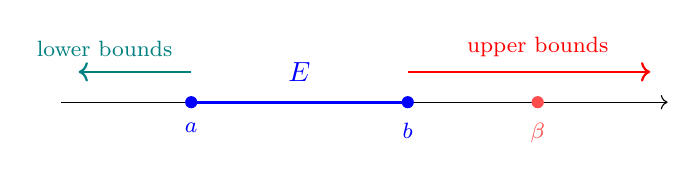
\begin{tikzpicture}[scale=1.1]
    % Number line
    \draw[->] (-0.5,0) -- (6.5,0);
    % Set E
    \draw[very thick, blue] (1,0) -- (3.5,0);
    \fill[blue] (1,0) circle (2pt) node[below=4pt]{\footnotesize$a$};
    \fill[blue] (3.5,0) circle (2pt) node[below=4pt]{\footnotesize$b$};
    \node[blue, above=4pt] at (2.25,0) {$E$};
    % Upper bounds
    \draw[thick, red, ->] (3.5,0.35) -- (6.3,0.35);
    \node[red, above=2pt] at (5.0,0.35) {\footnotesize upper bounds};
    % Lower bounds
    \draw[thick, teal, ->] (1,0.35) -- (-0.3,0.35);
    \node[teal, above=2pt] at (0.0,0.35) {\footnotesize lower bounds};
    % Example points
    \fill[red!70] (5,0) circle (2pt) node[below=4pt]{\footnotesize$\beta$};
  \end{tikzpicture}
  \end{center}

  \note{
    Here is the definition of an upper bound. Suppose S is an ordered
    set and E is a subset of S. If there is some element beta in S such
    that x is less than or equal to beta for every x in E, we say that
    E is bounded above, and we call beta an upper bound of E. As the
    diagram shows, upper bounds are elements that sit to the right of the
    entire set E. Lower bounds are defined symmetrically --- they sit to
    the left of E. Notice that the bound beta does not need to be in E
    itself; it just needs to be in S.
  }
\end{frame}

% ============================================================
\section{Supremum and Infimum}
% ============================================================

% --- Definition 1.8: Build 1/2 ---
\begin{frame}{Definition 1.8: Least Upper Bound (Supremum)}
  \begin{defblock}{Definition 1.8 --- Supremum}
    Let $S$ be an ordered set, $E \subset S$, $E$ bounded above. An element
    $\alpha \in S$ is the \alert{least upper bound} (or \alert{supremum}) of $E$ if:

    \vspace{0.3em}
    \textbf{(i)} $\alpha$ is an upper bound of $E$.
  \end{defblock}

  \note{
    Now we come to one of the most important definitions in this section:
    the supremum. Suppose E is a subset of an ordered set S and E is
    bounded above. The supremum of E is an element alpha in S satisfying
    two conditions. The first condition is that alpha must itself be an
    upper bound of E. But being an upper bound is not enough --- many
    elements could be upper bounds. The key is the second condition,
    which we will see on the next slide.
  }
\end{frame}

% --- Definition 1.8: Build 2/2 ---
\begin{frame}{Definition 1.8: Least Upper Bound (Supremum)}
  \begin{defblock}{Definition 1.8 --- Supremum}
    Let $S$ be an ordered set, $E \subset S$, $E$ bounded above. An element
    $\alpha \in S$ is the \alert{least upper bound} (or \alert{supremum}) of $E$ if:

    \vspace{0.3em}
    \textbf{(i)} $\alpha$ is an upper bound of $E$.

    \textbf{(ii)} If $\gamma < \alpha$, then $\gamma$ is \emph{not} an upper bound of $E$.
  \end{defblock}

  \vspace{0.3em}
  We write $\alpha = \sup E$.

  \begin{center}
  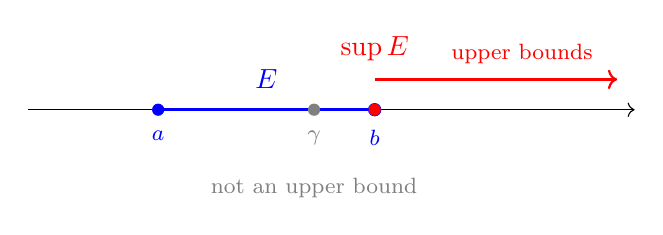
\begin{tikzpicture}[scale=1.1]
    \draw[->] (-0.5,0) -- (6.5,0);
    % Set E
    \draw[very thick, blue] (1,0) -- (3.5,0);
    \fill[blue] (1,0) circle (2pt) node[below=4pt]{\footnotesize$a$};
    \draw[blue] (3.5,0) circle (2pt) node[below=4pt]{\footnotesize$b$};
    \node[blue, above=4pt] at (2.25,0) {$E$};
    % Upper bounds region
    \draw[thick, red, ->] (3.5,0.35) -- (6.3,0.35);
    \node[red, above=2pt] at (5.2,0.35) {\footnotesize upper bounds};
    % Supremum
    \fill[red] (3.5,0) circle (2pt);
    \node[red, above=14pt] at (3.5,0) {$\sup E$};
    % gamma (not an upper bound)
    \fill[gray] (2.8,0) circle (2pt) node[below=4pt]{\footnotesize$\gamma$};
    \node[gray] at (2.8,-0.9) {\footnotesize not an upper bound};
  \end{tikzpicture}
  \end{center}

  \note{
    The second condition says that no element strictly smaller than alpha
    is an upper bound of E. In other words, alpha is the smallest of all
    upper bounds. That's why we call it the least upper bound. We write
    alpha equals sup E. Looking at the diagram, the supremum sits right
    at the boundary between E and the upper bounds. Any gamma to the left
    of it fails to be an upper bound because some element of E exceeds it.
    Notice from condition two that there is at most one supremum, since
    if two elements both satisfied these conditions, neither could be
    strictly less than the other.
  }
\end{frame}

% --- Infimum ---
\begin{frame}{Definition 1.8: Greatest Lower Bound (Infimum)}
  \begin{defblock}{Definition 1.8 --- Infimum}
    The \alert{greatest lower bound} (or \alert{infimum}) is defined symmetrically:
    $\alpha = \inf E$ means:

    \vspace{0.3em}
    \textbf{(i)} $\alpha$ is a lower bound of $E$.

    \textbf{(ii)} If $\beta > \alpha$, then $\beta$ is \emph{not} a lower bound of $E$.
  \end{defblock}

  \begin{center}
  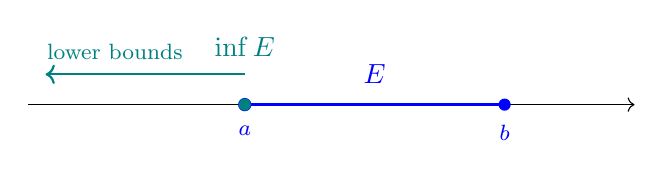
\begin{tikzpicture}[scale=1.1]
    \draw[->] (-0.5,0) -- (6.5,0);
    % Set E
    \draw[very thick, blue] (2,0) -- (5,0);
    \fill[blue] (5,0) circle (2pt) node[below=4pt]{\footnotesize$b$};
    \draw[blue] (2,0) circle (2pt) node[below=4pt]{\footnotesize$a$};
    \node[blue, above=4pt] at (3.5,0) {$E$};
    % Lower bounds region
    \draw[thick, teal, ->] (2,0.35) -- (-0.3,0.35);
    \node[teal, above=2pt] at (0.5,0.35) {\footnotesize lower bounds};
    % Infimum
    \fill[teal] (2,0) circle (2pt);
    \node[teal, above=14pt] at (2,0) {$\inf E$};
  \end{tikzpicture}
  \end{center}

  \note{
    The greatest lower bound, or infimum, is defined in the same manner
    but in the other direction. Alpha equals inf E means that alpha is a
    lower bound of E, and no beta strictly greater than alpha is a lower
    bound of E. So the infimum is the largest of all lower bounds. In
    the diagram, you can see the infimum sitting at the left boundary of
    E, with all lower bounds to its left. Now let's look at some examples
    to build intuition.
  }
\end{frame}

% ============================================================
\section{Examples}
% ============================================================

% --- Example 1.9(a) ---
\begin{frame}{Example 1.9(a): No Supremum in $\mathbb{Q}$}
  \begin{exblock}{Example 1.9(a)}
    Recall the sets from Example 1.1:
    \begin{align*}
      A &= \{p \in \mathbb{Q} : p > 0, \; p^2 < 2\} \\
      B &= \{p \in \mathbb{Q} : p > 0, \; p^2 > 2\}
    \end{align*}
  \end{exblock}

  \begin{center}
  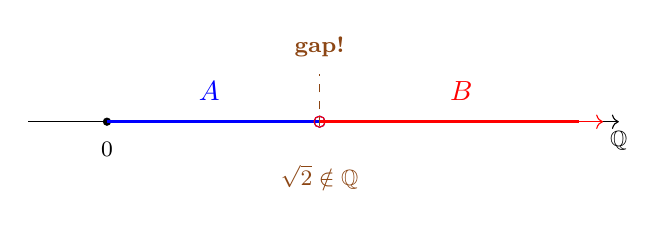
\begin{tikzpicture}[scale=1.0]
    \draw[->] (-0.5,0) -- (7,0);
    \node[below] at (7,0) {\footnotesize$\mathbb{Q}$};
    % Zero
    \fill (0.5,0) circle (1.5pt) node[below=4pt]{\footnotesize$0$};
    % Set A
    \draw[very thick, blue] (0.5,0) -- (3.2,0);
    \draw[blue] (3.2,0) circle (2pt);
    \node[blue, above=4pt] at (1.8,0) {$A$};
    % Set B
    \draw[very thick, red] (3.2,0) -- (6.5,0);
    \draw[red] (3.2,0) circle (2pt);
    \draw[red,->] (6.5,0) -- (6.8,0);
    \node[red, above=4pt] at (5.0,0) {$B$};
    % sqrt(2) gap
    \node[mAccent, below=12pt] at (3.2,0) {\footnotesize$\sqrt{2} \notin \mathbb{Q}$};
    \draw[mAccent,dashed] (3.2,-0.05) -- (3.2,0.6);
    \node[mAccent, above=20pt] at (3.2,0) {\footnotesize\textbf{gap!}};
  \end{tikzpicture}
  \end{center}

  \note{
    Let's revisit the sets from Example 1.1. The set A consists of all
    positive rationals whose square is less than 2, and B consists of all
    positive rationals whose square is greater than 2. On the number line,
    A lies to the left of the square root of 2, and B lies to the right.
    But the square root of 2 is not rational, so there is a gap between
    A and B. No rational number sits at the boundary.
  }
\end{frame}

% --- Example 1.9(a) continued ---
\begin{frame}{Example 1.9(a): No Supremum in $\mathbb{Q}$}
  \begin{exblock}{Example 1.9(a) --- Conclusion}
    \begin{itemize}
      \item The upper bounds of $A$ in $\mathbb{Q}$ are exactly the members of $B$.
      \item $B$ has no smallest member $\;\Longrightarrow\;$ \alert{$A$ has no supremum in $\mathbb{Q}$}
      \item The lower bounds of $B$ are $A$ and all $r \leq 0$. Since $A$ has no largest member, \alert{$B$ has no infimum in $\mathbb{Q}$}
    \end{itemize}
  \end{exblock}

  \note{
    The upper bounds of A within the rationals are exactly the members
    of B. Why? Any rational upper bound of A must satisfy p squared
    greater than or equal to 2, but since no rational has p squared equal
    to 2, it must satisfy p squared greater than 2, placing it in B. Now,
    B has no smallest member, as we proved in the introduction. That means
    there is no least upper bound for A within the rationals. A has no
    supremum in Q. Similarly, the lower bounds of B consist of all members
    of A together with all non-positive rationals. Since A has no largest
    member, B has no greatest lower bound in Q either. This is the
    fundamental gap that motivates everything that follows.
  }
\end{frame}

% --- Example 1.9(b): Build 1/2 ---
\begin{frame}{Example 1.9(b): Supremum May or May Not Belong to $E$}
  \begin{exblock}{Example 1.9(b)}
    If $\alpha = \sup E$ exists, $\alpha$ may or may not be a member of $E$.
  \end{exblock}

  \vspace{0.3em}
  Let $E_1 = \{r \in \mathbb{Q} : r < 0\}$ and $E_2 = \{r \in \mathbb{Q} : r \leq 0\}$.

  \begin{center}
  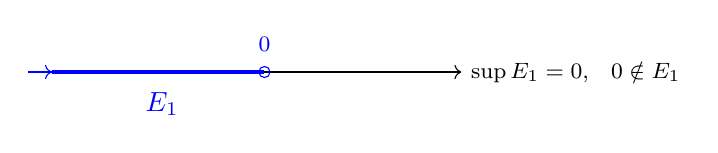
\begin{tikzpicture}[scale=1.0]
    % E_1
    \draw[->] (-0.5,0.8) -- (5,0.8);
    \draw[very thick, blue] (-0.2,0.8) -- (2.5,0.8);
    \draw[blue] (2.5,0.8) circle (2pt) node[above=4pt]{\footnotesize$0$};
    \node[blue, below=4pt] at (1.2,0.8) {$E_1$};
    \node[right] at (5,0.8) {\footnotesize$\sup E_1 = 0$, \; $0 \notin E_1$};
    \draw[blue, <-] (-0.2,0.8) -- (-0.5,0.8);
  \end{tikzpicture}
  \end{center}

  \note{
    An important point: the supremum of a set may or may not actually
    belong to that set. Consider E sub 1, the set of all rationals
    strictly less than 0. The supremum is 0, but 0 is not in E sub 1,
    because we required strict inequality.
  }
\end{frame}

% --- Example 1.9(b): Build 2/2 ---
\begin{frame}{Example 1.9(b): Supremum May or May Not Belong to $E$}
  \begin{exblock}{Example 1.9(b)}
    If $\alpha = \sup E$ exists, $\alpha$ may or may not be a member of $E$.
  \end{exblock}

  \vspace{0.3em}
  Let $E_1 = \{r \in \mathbb{Q} : r < 0\}$ and $E_2 = \{r \in \mathbb{Q} : r \leq 0\}$.

  \begin{center}
  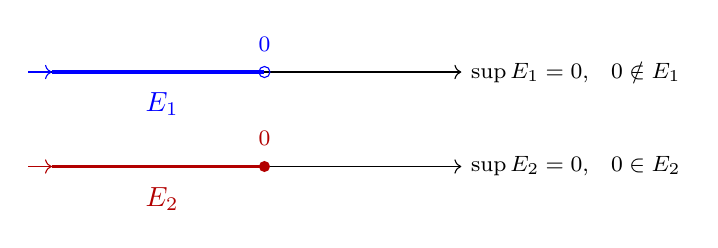
\begin{tikzpicture}[scale=1.0]
    % E_1
    \draw[->] (-0.5,1.2) -- (5,1.2);
    \draw[very thick, blue] (-0.2,1.2) -- (2.5,1.2);
    \draw[blue] (2.5,1.2) circle (2pt) node[above=4pt]{\footnotesize$0$};
    \node[blue, below=4pt] at (1.2,1.2) {$E_1$};
    \node[right] at (5,1.2) {\footnotesize$\sup E_1 = 0$, \; $0 \notin E_1$};
    \draw[blue, <-] (-0.2,1.2) -- (-0.5,1.2);
    % E_2
    \draw[->] (-0.5,0) -- (5,0);
    \draw[very thick, red!70!black] (-0.2,0) -- (2.5,0);
    \fill[red!70!black] (2.5,0) circle (2pt) node[above=4pt]{\footnotesize$0$};
    \node[red!70!black, below=4pt] at (1.2,0) {$E_2$};
    \node[right] at (5,0) {\footnotesize$\sup E_2 = 0$, \; $0 \in E_2$};
    \draw[red!70!black, <-] (-0.2,0) -- (-0.5,0);
  \end{tikzpicture}
  \end{center}

  \vspace{0.3em}
  Both have $\sup = 0$, but membership differs.

  \note{
    Now consider E sub 2, the set of all rationals less than or equal to
    zero. The supremum is again 0, but this time 0 belongs to E sub 2.
    The open circle on the E sub 1 diagram shows that 0 is excluded, while
    the filled circle for E sub 2 shows inclusion. Both sets have the same
    supremum, but membership differs. This is an important subtlety: the
    supremum need not be an element of the set.
  }
\end{frame}

% --- Example 1.9(c) ---
\begin{frame}{Example 1.9(c): The Set $\{1/n\}$}
  \begin{exblock}{Example 1.9(c)}
    Let $E = \{1/n : n = 1, 2, 3, \dots\} = \{1,\; 1/2,\; 1/3,\; 1/4,\; \dots\}$
  \end{exblock}

  \begin{center}
  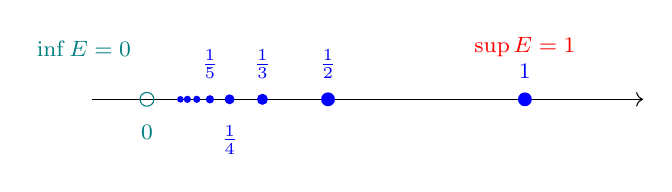
\begin{tikzpicture}[scale=1.0]
    \draw[->] (-0.5,0) -- (6.5,0);
    % Points
    \fill[blue] (5,0) circle (2.5pt) node[above=4pt]{\footnotesize$1$};
    \fill[blue] (2.5,0) circle (2.5pt) node[above=4pt]{\footnotesize$\tfrac{1}{2}$};
    \fill[blue] (1.667,0) circle (2pt) node[above=4pt]{\footnotesize$\tfrac{1}{3}$};
    \fill[blue] (1.25,0) circle (1.8pt) node[below=6pt]{\footnotesize$\tfrac{1}{4}$};
    \fill[blue] (1.0,0) circle (1.5pt) node[above=4pt]{\footnotesize$\tfrac{1}{5}$};
    \fill[blue] (0.833,0) circle (1.3pt);
    \fill[blue] (0.714,0) circle (1.3pt);
    \fill[blue] (0.625,0) circle (1.2pt);
    % Zero
    \draw[teal] (0.2,0) circle (2.5pt) node[below=6pt]{\footnotesize$0$};
    % Annotations
    \node[teal, above=12pt] at (-0.6,0) {\footnotesize$\inf E = 0$};
    \node[red, above=12pt] at (5,0) {\footnotesize$\sup E = 1$};
  \end{tikzpicture}
  \end{center}

  \vspace{0.3em}
  $\sup E = 1 \in E$, \quad $\inf E = 0 \notin E$.

  \note{
    Here is another instructive example. Let E be the set of all
    numbers 1 over n, where n ranges over the positive integers. So E
    is the set containing 1, one half, one third, one fourth, and so on.
    The supremum is 1, which is a member of E since 1 equals 1 over 1.
    The infimum is 0, which is not a member of E because there is no
    positive integer n with 1 over n equal to 0. The elements of E get
    closer and closer to 0, accumulating near it, but never reaching it.
    This example again illustrates that the supremum can belong to the
    set while the infimum does not, or vice versa.
  }
\end{frame}

% ============================================================
\section{The Least-Upper-Bound Property}
% ============================================================

% --- Definition 1.10 ---
\begin{frame}{Definition 1.10: Least-Upper-Bound Property}
  \begin{defblock}{Definition 1.10 --- Least-Upper-Bound Property}
    An ordered set $S$ has the \alert{least-upper-bound property} if:

    \vspace{0.3em}
    Whenever $E \subset S$, $E \neq \varnothing$, and $E$ is bounded above,
    then $\sup E$ exists in $S$.
  \end{defblock}

  \vspace{0.5em}
  Example 1.9(a) shows: \alert{$\mathbb{Q}$ does \emph{not} have the least-upper-bound property.}

  \note{
    This is one of the most important definitions in the book. An
    ordered set S has the least-upper-bound property if every nonempty
    subset of S that is bounded above has a supremum that exists within S.
    We already saw in Example 1.9 part a that the rationals do not have
    this property, because the set A of rationals with p squared less
    than 2 is bounded above but has no supremum in Q. In the next
    section, we will see that the real numbers are constructed precisely
    to have this property. But first, let's see an important consequence:
    the least-upper-bound property implies the greatest-lower-bound property.
  }
\end{frame}

% ============================================================
\section{Theorem 1.11 and Proof}
% ============================================================

% --- Theorem 1.11 statement ---
\begin{frame}{Theorem 1.11: LUB Property Implies GLB Property}
  \begin{thmblock}{Theorem 1.11}
    Suppose $S$ is an ordered set with the least-upper-bound property, $B \subset S$,
    $B \neq \varnothing$, and $B$ is bounded below. Let $L$ be the set of all lower bounds of $B$.

    \vspace{0.3em}
    Then $\alpha = \sup L$ exists in $S$, and $\alpha = \inf B$.

    \vspace{0.3em}
    \emph{In particular,} $\inf B$ exists in $S$.
  \end{thmblock}

  \note{
    Here is Theorem 1.11, which establishes a beautiful connection. If
    an ordered set S has the least-upper-bound property, then it also has
    the greatest-lower-bound property. More precisely, if B is a nonempty
    subset of S that is bounded below, and L is the set of all lower bounds
    of B, then the supremum of L exists and equals the infimum of B.
    This means we get greatest lower bounds for free once we have least
    upper bounds. Let's see why.
  }
\end{frame}

% --- Proof Strategy ---
\begin{frame}{Proof Strategy: Theorem 1.11}
  \textbf{Goal:} Show $\sup L = \inf B$, where $L = \{\text{lower bounds of } B\}$.

  \vspace{0.8em}
  \textbf{Approach:}
  \begin{enumerate}
    \item Show $L$ is nonempty and bounded above $\Longrightarrow$ $\sup L$ exists.
    \item Show $\alpha = \sup L$ is a lower bound of $B$ (i.e., $\alpha \in L$).
    \item Show nothing larger than $\alpha$ is a lower bound of $B$.
    \item Conclude $\alpha = \inf B$.
  \end{enumerate}

  \begin{center}
  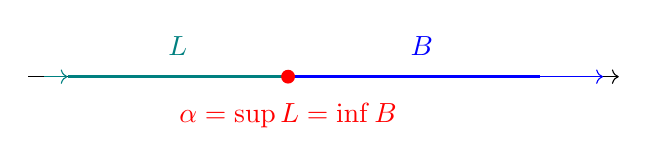
\begin{tikzpicture}[scale=1.0]
    \draw[->] (-0.5,0) -- (7,0);
    % L region
    \draw[very thick, teal] (0,0) -- (2.8,0);
    \draw[teal,<-] (0,0) -- (-0.3,0);
    \node[teal, above=4pt] at (1.4,0) {$L$};
    % B region
    \draw[very thick, blue] (2.8,0) -- (6,0);
    \draw[blue,->] (6,0) -- (6.8,0);
    \node[blue, above=4pt] at (4.5,0) {$B$};
    % alpha
    \fill[red] (2.8,0) circle (2.5pt);
    \node[red, below=6pt] at (2.8,0) {$\alpha = \sup L = \inf B$};
  \end{tikzpicture}
  \end{center}

  \note{
    Before we dive into the formal proof, let's understand the strategy.
    We have the set B, which is bounded below, and L, the set of all
    lower bounds of B. The picture shows L to the left and B to the right,
    with alpha at the boundary. Our plan is: first, use the
    least-upper-bound property to show that sup L exists. Then show that
    this supremum is actually a lower bound of B, meaning it belongs to L.
    Finally, show that nothing bigger than alpha is a lower bound of B.
    That will make alpha the greatest lower bound, the infimum of B.
  }
\end{frame}

% --- Proof Step 1 ---
\begin{frame}{Proof of Theorem 1.11 --- Step 1: $\sup L$ Exists}
  \begin{proofblock}{Step 1: $L$ is nonempty and bounded above}
    \begin{itemize}
      \item $B$ is bounded below $\;\Longrightarrow\;$ $L \neq \varnothing$.
      \item Every $x \in B$ is an upper bound of $L$ (since $y \leq x$ for all $y \in L$, $x \in B$).
      \item $L$ is bounded above $\;\Longrightarrow\;$ $\sup L$ exists in $S$ (by the LUB property).
    \end{itemize}

    Call this supremum $\alpha = \sup L$.
  \end{proofblock}

  \note{
    Let's begin. Since B is bounded below, there exists at least one lower
    bound, so L is not empty. Now, every element x of B is an upper bound
    for L. Why? Because L consists of all lower bounds of B, meaning every
    element of L is less than or equal to every element of B. So every
    element of B bounds L from above. Since L is nonempty and bounded
    above, and S has the least-upper-bound property, sup L must exist in S.
    Call it alpha.
  }
\end{frame}

% --- Proof Step 2 ---
\begin{frame}{Proof of Theorem 1.11 --- Step 2: $\alpha$ Is a Lower Bound of $B$}
  \begin{proofblock}{Step 2: $\alpha \in L$}
    Take any $x \in B$. Since $x$ is an upper bound of $L$ and $\alpha = \sup L$:
    \[
      \alpha \leq x \quad \text{for every } x \in B.
    \]
    Therefore $\alpha$ is a lower bound of $B$, i.e., $\alpha \in L$.
  \end{proofblock}

  \note{
    Now we show that alpha is actually a lower bound of B. Take any
    element x in B. We just showed that x is an upper bound of L. Since
    alpha is the least upper bound of L, alpha must be less than or equal
    to x. But x was arbitrary in B. So alpha is less than or equal to
    every element of B, which means alpha is a lower bound of B. In
    other words, alpha belongs to L. Now we just need to show that
    nothing larger than alpha is also a lower bound of B.
  }
\end{frame}

% --- Proof Step 3 ---
\begin{frame}{Proof of Theorem 1.11 --- Step 3: $\alpha$ Is the Greatest Lower Bound}
  \begin{proofblock}{Step 3: No $\beta > \alpha$ is a lower bound of $B$}
    If $\alpha < \beta$, then $\beta \notin L$.

    \vspace{0.3em}
    \emph{Why?} $\alpha$ is an upper bound of $L$, so every $y \in L$ satisfies
    $y \leq \alpha < \beta$. If $\beta$ were in $L$, we'd need $\beta \leq \alpha$ --- contradiction.
  \end{proofblock}

  \vspace{0.5em}
  \textbf{Conclusion:}
  \begin{itemize}
    \item $\alpha$ is a lower bound of $B$ \hfill (Step 2)
    \item No $\beta > \alpha$ is a lower bound of $B$ \hfill (Step 3)
  \end{itemize}

  \vspace{0.3em}
  $\boxed{\alpha = \inf B}$

  \note{
    Finally, suppose beta is strictly greater than alpha. Since alpha is
    the supremum of L, every element of L is at most alpha. So if beta
    were in L, we would need beta less than or equal to alpha, which
    contradicts beta being strictly greater. Therefore beta is not in L,
    meaning beta is not a lower bound of B. Putting it all together:
    alpha is a lower bound of B from Step 2, and no element greater than
    alpha is a lower bound of B from Step 3. By definition, this means
    alpha equals the infimum of B. The proof is complete. This elegant
    argument shows that the least-upper-bound property automatically
    gives us the greatest-lower-bound property as well.
  }
\end{frame}

% ============================================================
\section{Summary}
% ============================================================

% --- Summary: Build 1/4 ---
\begin{frame}{Summary}
  \textbf{Key takeaways from this section:}
  \begin{itemize}
    \item An \alert{order} on a set requires trichotomy and transitivity (Def.\ 1.5--1.6)
  \end{itemize}

  \note{
    Let's review what we covered. First, we defined what an order is:
    a relation satisfying trichotomy, meaning every pair of elements is
    comparable in exactly one way, and transitivity, meaning the relation
    chains consistently.
  }
\end{frame}

% --- Summary: Build 2/4 ---
\begin{frame}{Summary}
  \textbf{Key takeaways from this section:}
  \begin{itemize}
    \item An \alert{order} on a set requires trichotomy and transitivity (Def.\ 1.5--1.6)
    \item The \alert{supremum} is the least upper bound; the \alert{infimum} is the greatest lower bound (Def.\ 1.7--1.8)
  \end{itemize}

  \note{
    Second, we defined upper and lower bounds, and introduced the
    supremum and infimum as the tightest possible bounds. The supremum
    may or may not belong to the set.
  }
\end{frame}

% --- Summary: Build 3/4 ---
\begin{frame}{Summary}
  \textbf{Key takeaways from this section:}
  \begin{itemize}
    \item An \alert{order} on a set requires trichotomy and transitivity (Def.\ 1.5--1.6)
    \item The \alert{supremum} is the least upper bound; the \alert{infimum} is the greatest lower bound (Def.\ 1.7--1.8)
    \item $\mathbb{Q}$ lacks the \alert{least-upper-bound property} (Ex.\ 1.9, Def.\ 1.10)
  \end{itemize}

  \note{
    Third, we saw concretely that the rationals do not have the
    least-upper-bound property. The set of rationals whose square is
    less than 2 is bounded above but has no supremum in the rationals.
  }
\end{frame}

% --- Summary: Build 4/4 ---
\begin{frame}{Summary}
  \textbf{Key takeaways from this section:}
  \begin{itemize}
    \item An \alert{order} on a set requires trichotomy and transitivity (Def.\ 1.5--1.6)
    \item The \alert{supremum} is the least upper bound; the \alert{infimum} is the greatest lower bound (Def.\ 1.7--1.8)
    \item $\mathbb{Q}$ lacks the \alert{least-upper-bound property} (Ex.\ 1.9, Def.\ 1.10)
    \item LUB property $\Longrightarrow$ GLB property (Thm.\ 1.11)
  \end{itemize}

  \vspace{1em}
  \textbf{Coming up next:} Fields --- the algebraic structure of $\mathbb{Q}$ and $\mathbb{R}$.

  \note{
    And finally, Theorem 1.11 showed that the least-upper-bound property
    automatically implies the greatest-lower-bound property. So once we
    construct the real numbers with the least-upper-bound property, we
    get infima for free as well. In the next section, we will study
    fields, which capture the algebraic structure --- addition and
    multiplication --- of the rational and real numbers. See you there.
  }
\end{frame}

\end{document}
